% Options for packages loaded elsewhere
\PassOptionsToPackage{unicode}{hyperref}
\PassOptionsToPackage{hyphens}{url}
\PassOptionsToPackage{dvipsnames,svgnames,x11names}{xcolor}
%
\documentclass[
  10pt,
]{article}
\usepackage{amsmath,amssymb}
\usepackage{iftex}
\ifPDFTeX
  \usepackage[T1]{fontenc}
  \usepackage[utf8]{inputenc}
  \usepackage{textcomp} % provide euro and other symbols
\else % if luatex or xetex
  \usepackage{unicode-math} % this also loads fontspec
  \defaultfontfeatures{Scale=MatchLowercase}
  \defaultfontfeatures[\rmfamily]{Ligatures=TeX,Scale=1}
\fi
\usepackage{lmodern}
\ifPDFTeX\else
  % xetex/luatex font selection
  \setmainfont[]{DejaVu Serif}
  \setsansfont[]{DejaVu Sans}
  \setmonofont[]{DejaVu Sans Mono}
  \setmathfont[]{Latin Modern Math}
\fi
% Use upquote if available, for straight quotes in verbatim environments
\IfFileExists{upquote.sty}{\usepackage{upquote}}{}
\IfFileExists{microtype.sty}{% use microtype if available
  \usepackage[]{microtype}
  \UseMicrotypeSet[protrusion]{basicmath} % disable protrusion for tt fonts
}{}
\makeatletter
\@ifundefined{KOMAClassName}{% if non-KOMA class
  \IfFileExists{parskip.sty}{%
    \usepackage{parskip}
  }{% else
    \setlength{\parindent}{0pt}
    \setlength{\parskip}{6pt plus 2pt minus 1pt}}
}{% if KOMA class
  \KOMAoptions{parskip=half}}
\makeatother
\usepackage{xcolor}
\usepackage[margin=2.0cm]{geometry}
\usepackage{color}
\usepackage{fancyvrb}
\newcommand{\VerbBar}{|}
\newcommand{\VERB}{\Verb[commandchars=\\\{\}]}
\DefineVerbatimEnvironment{Highlighting}{Verbatim}{commandchars=\\\{\}}
% Add ',fontsize=\small' for more characters per line
\newenvironment{Shaded}{}{}
\newcommand{\AlertTok}[1]{\textcolor[rgb]{1.00,0.00,0.00}{\textbf{#1}}}
\newcommand{\AnnotationTok}[1]{\textcolor[rgb]{0.38,0.63,0.69}{\textbf{\textit{#1}}}}
\newcommand{\AttributeTok}[1]{\textcolor[rgb]{0.49,0.56,0.16}{#1}}
\newcommand{\BaseNTok}[1]{\textcolor[rgb]{0.25,0.63,0.44}{#1}}
\newcommand{\BuiltInTok}[1]{\textcolor[rgb]{0.00,0.50,0.00}{#1}}
\newcommand{\CharTok}[1]{\textcolor[rgb]{0.25,0.44,0.63}{#1}}
\newcommand{\CommentTok}[1]{\textcolor[rgb]{0.38,0.63,0.69}{\textit{#1}}}
\newcommand{\CommentVarTok}[1]{\textcolor[rgb]{0.38,0.63,0.69}{\textbf{\textit{#1}}}}
\newcommand{\ConstantTok}[1]{\textcolor[rgb]{0.53,0.00,0.00}{#1}}
\newcommand{\ControlFlowTok}[1]{\textcolor[rgb]{0.00,0.44,0.13}{\textbf{#1}}}
\newcommand{\DataTypeTok}[1]{\textcolor[rgb]{0.56,0.13,0.00}{#1}}
\newcommand{\DecValTok}[1]{\textcolor[rgb]{0.25,0.63,0.44}{#1}}
\newcommand{\DocumentationTok}[1]{\textcolor[rgb]{0.73,0.13,0.13}{\textit{#1}}}
\newcommand{\ErrorTok}[1]{\textcolor[rgb]{1.00,0.00,0.00}{\textbf{#1}}}
\newcommand{\ExtensionTok}[1]{#1}
\newcommand{\FloatTok}[1]{\textcolor[rgb]{0.25,0.63,0.44}{#1}}
\newcommand{\FunctionTok}[1]{\textcolor[rgb]{0.02,0.16,0.49}{#1}}
\newcommand{\ImportTok}[1]{\textcolor[rgb]{0.00,0.50,0.00}{\textbf{#1}}}
\newcommand{\InformationTok}[1]{\textcolor[rgb]{0.38,0.63,0.69}{\textbf{\textit{#1}}}}
\newcommand{\KeywordTok}[1]{\textcolor[rgb]{0.00,0.44,0.13}{\textbf{#1}}}
\newcommand{\NormalTok}[1]{#1}
\newcommand{\OperatorTok}[1]{\textcolor[rgb]{0.40,0.40,0.40}{#1}}
\newcommand{\OtherTok}[1]{\textcolor[rgb]{0.00,0.44,0.13}{#1}}
\newcommand{\PreprocessorTok}[1]{\textcolor[rgb]{0.74,0.48,0.00}{#1}}
\newcommand{\RegionMarkerTok}[1]{#1}
\newcommand{\SpecialCharTok}[1]{\textcolor[rgb]{0.25,0.44,0.63}{#1}}
\newcommand{\SpecialStringTok}[1]{\textcolor[rgb]{0.73,0.40,0.53}{#1}}
\newcommand{\StringTok}[1]{\textcolor[rgb]{0.25,0.44,0.63}{#1}}
\newcommand{\VariableTok}[1]{\textcolor[rgb]{0.10,0.09,0.49}{#1}}
\newcommand{\VerbatimStringTok}[1]{\textcolor[rgb]{0.25,0.44,0.63}{#1}}
\newcommand{\WarningTok}[1]{\textcolor[rgb]{0.38,0.63,0.69}{\textbf{\textit{#1}}}}
\usepackage{longtable,booktabs,array}
\usepackage{calc} % for calculating minipage widths
% Correct order of tables after \paragraph or \subparagraph
\usepackage{etoolbox}
\makeatletter
\patchcmd\longtable{\par}{\if@noskipsec\mbox{}\fi\par}{}{}
\makeatother
% Allow footnotes in longtable head/foot
\IfFileExists{footnotehyper.sty}{\usepackage{footnotehyper}}{\usepackage{footnote}}
\makesavenoteenv{longtable}
\usepackage{graphicx}
\makeatletter
\def\maxwidth{\ifdim\Gin@nat@width>\linewidth\linewidth\else\Gin@nat@width\fi}
\def\maxheight{\ifdim\Gin@nat@height>\textheight\textheight\else\Gin@nat@height\fi}
\makeatother
% Scale images if necessary, so that they will not overflow the page
% margins by default, and it is still possible to overwrite the defaults
% using explicit options in \includegraphics[width, height, ...]{}
\setkeys{Gin}{width=\maxwidth,height=\maxheight,keepaspectratio}
% Set default figure placement to htbp
\makeatletter
\def\fps@figure{htbp}
\makeatother
\setlength{\emergencystretch}{3em} % prevent overfull lines
\providecommand{\tightlist}{%
  \setlength{\itemsep}{0pt}\setlength{\parskip}{0pt}}
\setcounter{secnumdepth}{-\maxdimen} % remove section numbering
% doc_header.tex -- LaTeX preamble additions used by build_docs.sh for every
% Markdown -> LaTeX -> PDF conversion (supplements, README, submission files).
\usepackage{etoolbox}
% longtable may not be loaded by pandoc when a document has no table
\usepackage{longtable}
% bold vectors: \bm -> \symbf under unicode-math (XeLaTeX), bm package otherwise
\makeatletter
\@ifpackageloaded{unicode-math}{\providecommand{\bm}[1]{\symbf{#1}}}{\usepackage{bm}}
\makeatother
% smaller type in long tables so that wide audit tables fit the text width;
% inside a table a line break is allowed after an underscore of plain text
% (pandoc writes it as \_), so that long identifiers wrap inside their column
% rows are set a little apart, so that symbols with indices do not touch
\AtBeginEnvironment{longtable}{\footnotesize\renewcommand{\arraystretch}{1.45}%
  \let\sptunderscore\_\def\_{\sptunderscore\allowbreak}}
\setlength{\LTcapwidth}{\textwidth}
% allow line breaks after slashes and hyphens inside table cells
\usepackage{xurl}
% code blocks: break over-long lines instead of running into the margin.
% Plain ``` blocks are typeset by pandoc as {verbatim}, highlighted ones
% (```bash) as {Highlighting}; both are re-declared as breakable fancyvrb
% environments.  The continuation line is marked with a small hooked arrow.
\usepackage{fvextra}
\RecustomVerbatimEnvironment{verbatim}{Verbatim}{breaklines,breakanywhere,fontsize=\small}
\makeatletter
\@ifundefined{Highlighting}{}{%
  \RecustomVerbatimEnvironment{Highlighting}{Verbatim}{breaklines,breakanywhere,fontsize=\small,commandchars=\\\{\}}}
\makeatother
% inline code (pandoc writes it as \texttt{...}): never hyphenate -- an inserted
% hyphen could be read as part of a file name -- but allow a line break after
% an underscore, slash, comma, colon or equals sign, so that long paths and
% column lists wrap inside the text width and inside table columns.
% Inside a formula (e.g. the name of a notebook symbol in an equation) the same
% command must first leave math mode, which \text of amsmath does.
\ExplSyntaxOn
\tl_new:N \l__spt_code_tl
\cs_new_protected:Npn \__spt_texttt:n #1
  {
    \tl_set:Nn \l__spt_code_tl {#1}
    \regex_replace_all:nnN { ([\/\,\:\=]) } { \1 \c{allowbreak} } \l__spt_code_tl
    \regex_replace_all:nnN { \c{_} } { \c{_} \c{allowbreak} } \l__spt_code_tl
    \group_begin: \ttfamily \hyphenchar \font = -1 \scan_stop: \l__spt_code_tl \group_end:
  }
\RenewDocumentCommand \texttt { m }
  {
    \mode_if_math:TF { \text { \__spt_texttt:n {#1} } } { \__spt_texttt:n {#1} }
  }
\ExplSyntaxOff
% A figure is written in the Markdown source as an image paragraph followed by
% a caption paragraph ("**Figure S1.** ..."), so that the caption is also
% visible on GitHub.  An image that starts a paragraph is centered.
\usepackage{graphicx}% pandoc loads it only for documents that contain an image
\NewCommandCopy\sptincludegraphics\includegraphics
\RenewDocumentCommand\includegraphics{O{} m}{%
  \ifvmode\begin{center}\sptincludegraphics[#1]{#2}\end{center}%
  \else\sptincludegraphics[#1]{#2}\fi}
% keep figures where they are referenced
\usepackage{float}
\floatplacement{figure}{H}
% running header with the document title
\usepackage{fancyhdr}
\pagestyle{fancy}
\fancyhf{}
\fancyhead[L]{\small PROJECT spacetimes, Revision\_Deflation --- documentation and provenance}
\fancyhead[R]{\small\thepage}
\renewcommand{\headrulewidth}{0.4pt}
% 16x16 matrices: tighter columns so that a full matrix fits the text width
\setlength{\arraycolsep}{3.2pt}
% The documents of this project contain long tagged symbols, file paths and
% identifiers that cannot be hyphenated.  A paragraph is therefore allowed to
% have looser lines before TeX gives up and lets a line stick out of the margin.
\AtBeginDocument{\tolerance=2000 \emergencystretch=5em \hbadness=2000}
\ifLuaTeX
  \usepackage{selnolig}  % disable illegal ligatures
\fi
\IfFileExists{bookmark.sty}{\usepackage{bookmark}}{\usepackage{hyperref}}
\IfFileExists{xurl.sty}{\usepackage{xurl}}{} % add URL line breaks if available
\urlstyle{same}
\hypersetup{
  pdftitle={RS3 --- Cosmology on the deflating spacetimes: bounds on the rate of deflation, dark matter, and the Hubble tension},
  pdfauthor={Prepared for Patrick Lee Nash, Ph.D.},
  colorlinks=true,
  linkcolor={blue},
  filecolor={Maroon},
  citecolor={blue},
  urlcolor={blue},
  pdfcreator={LaTeX via pandoc}}

\title{RS3 --- Cosmology on the deflating spacetimes: bounds on the rate
of deflation, dark matter, and the Hubble tension}
\usepackage{etoolbox}
\makeatletter
\providecommand{\subtitle}[1]{% add subtitle to \maketitle
  \apptocmd{\@title}{\par {\large #1 \par}}{}{}
}
\makeatother
\subtitle{PROJECT spacetimes, Revision\_Deflation. Supplement to both
manuscripts of the revision}
\author{Prepared for Patrick Lee Nash, Ph.D.}
\date{November 12, 2026}

\begin{document}
\maketitle

\hypertarget{purpose-and-summary}{%
\section{0. Purpose and summary}\label{purpose-and-summary}}

The author's task poses two cosmological hypotheses about the superfluid
of the 16-component field: that it is the dark matter, and that it
resolves the Hubble tension. The supplement S3 of the main project
examines both on flat extra dimensions. This supplement examines what
changes when the coordinates \(x5\), \(x6\), \(x7\) deflate.

The deflation enters cosmology in several ways, each of which requires
an assumption beyond the hypotheses of the revision. The assumptions are
stated in Sec. 1 and are kept apart throughout, so that the reader can
see which conclusion rests on which.

\textbf{Summary.}

\begin{enumerate}
\def\labelenumi{\arabic{enumi}.}
\tightlist
\item
  \emph{If gravity is eight-dimensional} (assumption A2), Newton's
  constant grows at the rate of the deflation. Lunar laser ranging then
  bounds the present rate to \(\mathrm{gsum}<3.24\times10^{-3}\,H_0\):
  over the age of the universe every coupling of the model has changed
  by less than a third of a per cent. \emph{If the superfluid is the
  Higgs field} (the author's hypothesis H2), atomic clocks bound the
  rate about three thousand times more strongly still. In either case
  nothing that the supplements RS1 and RS4 describe along the deflation
  clock can have happened within cosmic history at a constant rate (Sec.
  3).
\item
  \emph{The Hubble tension is not relieved.} With A2 the Hubble constant
  inferred from the sound horizon \textbf{falls}, away from the locally
  measured value, by 0.2 km/s/Mpc at the largest allowed rate (Sec. 2).
  Without A2 the only effect of the deflation that raises it is the loss
  of rest mass of bound pairs, which supplies at most \(+0.48\) km/s/Mpc
  in the examples computed (Sec. 4).
\item
  \emph{Dark matter.} The estimates of the main project that involve
  masses only are unchanged. New is an epoch: the moment at which the
  pairs become bound is a scattering resonance, during which the
  self-interaction of the fermions exceeds the observational bound by
  many orders of magnitude (Sec. 6). The growth of structure changes
  little in amplitude and more in rate (Sec. 5).
\item
  \emph{The particles that the deflation creates} (7+1) have a
  temperature of \(2.9\times10^{-33}\) K at the rate that lunar laser
  ranging allows, and below \(10^{-30}\) K at any allowed rate: none are
  created today (Sec. 7).
\item
  \emph{Not done.} The spectra of the microwave background, which S3
  computes with its own Einstein--Boltzmann program, have not been
  recomputed with a time-dependent Newton's constant. The reason and the
  consequence are stated in Sec. 9.
\end{enumerate}

\hypertarget{how-to-reproduce}{%
\subsection{0.1 How to reproduce}\label{how-to-reproduce}}

\begin{Shaded}
\begin{Highlighting}[]
\BuiltInTok{cd} \StringTok{"/Users/nsh/Developer/github/spacetimes/Revision\_Deflation"}
\ExtensionTok{cargo}\NormalTok{ build }\AttributeTok{{-}{-}release} \AttributeTok{{-}{-}manifest{-}path}\NormalTok{ code/deflation{-}rs/Cargo.toml}
\ExtensionTok{./code/deflation{-}rs/target/release/deflation}\NormalTok{ cosmology   }\CommentTok{\# Secs. 2 to 4 (about a minute)}
\ExtensionTok{./code/deflation{-}rs/target/release/deflation}\NormalTok{ matter      }\CommentTok{\# Secs. 5 to 7}
\ExtensionTok{python3}\NormalTok{ code/scripts/make\_figures.py hubble bounds binding}
\ExtensionTok{python3}\NormalTok{ code/scripts/write\_doc\_tables.py}
\ExtensionTok{python3}\NormalTok{ code/scripts/assemble\_docs.py docs\_src/RS3\_cosmology\_deflating.src.md}
\FunctionTok{bash}\NormalTok{ code/scripts/build\_docs.sh supplement/RS3\_cosmology\_deflating.md}
\end{Highlighting}
\end{Shaded}

\hypertarget{symbols}{%
\subsection{0.2 Symbols}\label{symbols}}

\begin{longtable}[]{@{}
  >{\raggedright\arraybackslash}p{(\columnwidth - 8\tabcolsep) * \real{0.1379}}
  >{\raggedright\arraybackslash}p{(\columnwidth - 8\tabcolsep) * \real{0.1379}}
  >{\raggedright\arraybackslash}p{(\columnwidth - 8\tabcolsep) * \real{0.4483}}
  >{\raggedright\arraybackslash}p{(\columnwidth - 8\tabcolsep) * \real{0.1379}}
  >{\raggedright\arraybackslash}p{(\columnwidth - 8\tabcolsep) * \real{0.1379}}@{}}
\toprule\noalign{}
\begin{minipage}[b]{\linewidth}\raggedright
symbol
\end{minipage} & \begin{minipage}[b]{\linewidth}\raggedright
in programs and data files
\end{minipage} & \begin{minipage}[b]{\linewidth}\raggedright
meaning
\end{minipage} & \begin{minipage}[b]{\linewidth}\raggedright
defined in
\end{minipage} & \begin{minipage}[b]{\linewidth}\raggedright
origin
\end{minipage} \\
\midrule\noalign{}
\endhead
\bottomrule\noalign{}
\endlastfoot
\(G_N\), \(G_8\) & \texttt{G\_N}, \texttt{GN\_early}, \texttt{GN\_star},
\texttt{G\_8} & Newton's constant of ordinary space, and the
gravitational coupling of the eight-dimensional Einstein theory
(assumption A2):
\(G_N=G_8/(\text{proper volume of the extra coordinates})\propto e^{\mathrm{gsum}\,x4}\)
& RS3 1; M XI & new \\
\(a_{\rm sp}\), \(H\) & --- & scale factor of ordinary space (assumption
A1) and its rate \(H=(da_{\rm sp}/dx4)/a_{\rm sp}\); \(H_0\), \(h\) as
in the main registry. (The author's Einstein-Lovelock notebooks use the
letter \(H\) for the rate in the exponent of their metric; that rate
corresponds here to \(\mathrm{g55}\), \(\mathrm{g66}\),
\(\mathrm{g77}\)) & RS3 1; M XI & new \\
\(t_0\) & \texttt{age}, \texttt{age\_Gyr} & the age of the universe in
the model at hand & RS3 2; M XI & new \\
\(\theta_*\), \(z_*\) & \texttt{theta\_star}, \texttt{z\_star} & the
angle under which the sound horizon at last scattering is seen,
\(r_s(z_*)/D_A(z_*)\) with the comoving distance \(D_A\), and the
redshift \(z_*\) of last scattering at which the optical depth without
reionization is 1 (the \(100\,\theta_*\) of the Planck papers). The
angle \(\theta_s\) of the main registry is the same ratio at the maximum
of the visibility function; for the model without deflation
\(100\,\theta_*=1.03965\) and \(100\,\theta_s=1.040358\) & RS3 1, 2; M
XI & new \\
\(\delta_m\), \(f_g\), \(\sigma_8\) & \texttt{growth},
\texttt{f\_growth}, \texttt{growth\_ratio}, \texttt{f\_growth\_ratio},
\texttt{f\_sigma8\_ratio} & density contrast of matter in ordinary
space; its growth rate \(d\ln\delta_m/d\ln a_{\rm sp}\) today; the
amplitude of clustering (only ratios of \(\sigma_8\) are used) & RS3 5;
M XI & new \\
\(v_{\rm EW}\) (main project), \(n_{\rm EW}\) & \texttt{v\_EW},
\texttt{n\_EW} & the electroweak scale of the supplement S2 of the main
project, and the exponent with which it would follow the coupling under
the hypothesis H2: \(n_{\rm EW}=d\ln v_{\rm EW}/d\ln\alpha_{VS}\) & RS2
5; M XII & new \\
\(\varrho_c\) & \texttt{rho\_c} & abbreviation in the formula for
\(n_{\rm EW}\) of the scale-invariant ladder equation:
\(\varrho_c=\tfrac12\sqrt{\alpha_{VS}/\alpha_c-1}\) (the letter \(\rho\)
without index is a density) & RS2 5; M XII & new \\
\(m_p/m_e\) & \texttt{mu\_pe} & the ratio of the proton mass to the
electron mass (always written as this ratio in the documents;
\texttt{mu\_pe} in the statements of the programs) & RS2 5; RS3 3; M XI
& new \\
\(G_{\rm Fermi}\), \(\alpha_{\rm em}\) & \texttt{G\_Fermi} & the Fermi
constant of the weak interaction and the fine-structure constant (they
enter only in the discussion of bounds) & RS3 1, 3; M XI & new \\
\end{longtable}

\begin{center}\rule{0.5\linewidth}{0.5pt}\end{center}

\hypertarget{the-assumptions-and-the-equation-of-the-expansion}{%
\section{1. The assumptions, and the equation of the
expansion}\label{the-assumptions-and-the-equation-of-the-expansion}}

The author's hypotheses fix the metric of the three deflating
coordinates. Cosmology needs more. Of the following four statements, A1,
A2 and HV are assumptions of this supplement, and H2 is the author's
hypothesis of the main project; each is used only where stated.

\textbf{A1 --- ordinary space expands.} The coordinates \(x1,x2,x3\)
carry the scale factor \(a_{\rm sp}(x4)\) of standard cosmology, with
the Hubble rate \(H=d\ln a_{\rm sp}/dx4\); the hidden coordinate \(x0\)
is static; \(x5,x6,x7\) deflate at constant rates. (The metric of DMD is
the special case \(a_{\rm sp}=1\).)

\textbf{A2 --- gravity is eight-dimensional.} The metric obeys
Einstein's equations in eight dimensions with a constant \(G_8\). The
constant of gravitation that an observer in ordinary space measures is
then
\[G_N(x4)=\frac{G_8}{\text{volume of the extra coordinates}}\ \propto\ \frac1{V_d}\ \propto\ e^{\mathrm{gsum}\,x4},
\qquad\frac{1}{G_N}\frac{dG_N}{dx4}=\mathrm{gsum}.\tag{1.1}\] Newton's
constant \emph{grows} as the extra volume shrinks: gravity was weaker in
the past. (That a changing volume of extra dimensions makes the
constants of four dimensions change, and that nucleosynthesis bounds the
change, was pointed out in Ref. {[}5{]}.)

\textbf{H2 --- the author's hypothesis about the Higgs field.} The main
project calls H2 the hypothesis that the superfluid state --- the pair
condensate along the hidden axis --- is the Higgs field. If it holds,
the electroweak scale \(v_{\rm EW}\) is the scale of that condensate in
the vacuum, which depends on the coupling \(\alpha_{VS}\); and
\(\alpha_{VS}\) grows with the deflation. The supplement RS2, Sec. 5,
derives the consequence: the masses of the ordinary fermions follow
\(v_{\rm EW}\) and change at the rate \(n_{\rm EW}\,\mathrm{gsum}\),
with the exponent \(n_{\rm EW}=d\ln v_{\rm EW}/d\ln\alpha_{VS}\).

\textbf{HV --- the vacuum value of the Vorton-Scalar sets the
electroweak scale.} This is a \emph{different} assumption, not the
author's: the Vorton-Scalar itself plays the role of the Higgs field.
(The supplement S2 of the main project notes that the Vorton-Scalar, a
singlet of all non-Abelian symmetries, cannot be the Higgs field of the
Standard Model; the assumption is examined only to show what it would
imply.) Under HV the Fermi constant is
\(G_{\rm Fermi}=1/(\sqrt2\,v_{VS}^2)\) with the four-dimensional vacuum
value, and grows as \(e^{\tau_d}\), while every mass \(m=y\,v/\sqrt2\)
stays constant (RS1, Sec. 1.3).

\emph{The equation of the expansion.} For a diagonal metric whose seven
space-like or deflating directions have the rates \(H,H,H\) (ordinary
space), \(0\) (the coordinate \(x0\)) and
\(-\mathrm{g55},-\mathrm{g66},-\mathrm{g77}\), the component of
Einstein's equations along the time is the sum of the products of all
pairs of rates, set equal to \(8\pi G_8\) times the energy density in
eight dimensions. Dividing the density by the extra volume turns \(G_8\)
into \(G_N\):
\[\boxed{\;3H^2-3\,\mathrm{gsum}\,H+\mathrm{gprod}=8\pi\,G_N(x4)\,\rho\;}\tag{1.2}\]
with
\(\mathrm{gprod}=\mathrm{g55}\,\mathrm{g66}+\mathrm{g55}\,\mathrm{g77}+\mathrm{g66}\,\mathrm{g77}\)
and the density \(\rho\) of radiation, matter and the cosmological term
in ordinary space. For \(H=0\) and \(\rho\to\) the source of DMD, Sec.
1.4, this is the component \(\mathcal G^4{}_4\) computed there. Equation
(1.2) is the only one of Einstein's equations that this supplement uses;
the others would determine the stresses of the unknown source that keeps
the three rates constant (Sec. 9).

The calculations take three equal rates, so that
\(\mathrm{gprod}=\mathrm{gsum}^2/3\), and the densities of the model of
the main project without deflation (baryons \(\omega_b=0.02237\), cold
dark matter \(\omega_c=0.1200\), \(H_0=67.36\) km/s/Mpc); the
cosmological term is chosen so that Eq. (1.2) holds today. Without
deflation the program reproduces the angular scale of the sound horizon
and the sound horizon of the main project: \(100\,\theta_*=1.03965\) and
144.449 Mpc (check \texttt{def-C1}).

\begin{center}\rule{0.5\linewidth}{0.5pt}\end{center}

\hypertarget{the-hubble-constant-inferred-from-the-sound-horizon}{%
\section{2. The Hubble constant inferred from the sound
horizon}\label{the-hubble-constant-inferred-from-the-sound-horizon}}

The microwave background fixes, to high precision, the angle
\(\theta_*\) under which the sound horizon at last scattering is seen. A
model that changes the expansion history must keep that angle, and the
Hubble constant that it then requires is the ``inferred'' Hubble
constant. With A1 and A2, at fixed \(\theta_*\) and fixed densities of
baryons and dark matter (check \texttt{def-C2}; independently
\texttt{Idef-C1}):

\begin{longtable}[]{@{}
  >{\raggedleft\arraybackslash}p{(\columnwidth - 12\tabcolsep) * \real{0.1429}}
  >{\raggedleft\arraybackslash}p{(\columnwidth - 12\tabcolsep) * \real{0.1429}}
  >{\raggedleft\arraybackslash}p{(\columnwidth - 12\tabcolsep) * \real{0.1429}}
  >{\raggedleft\arraybackslash}p{(\columnwidth - 12\tabcolsep) * \real{0.1429}}
  >{\raggedleft\arraybackslash}p{(\columnwidth - 12\tabcolsep) * \real{0.1429}}
  >{\raggedleft\arraybackslash}p{(\columnwidth - 12\tabcolsep) * \real{0.1429}}
  >{\raggedleft\arraybackslash}p{(\columnwidth - 12\tabcolsep) * \real{0.1429}}@{}}
\toprule\noalign{}
\begin{minipage}[b]{\linewidth}\raggedleft
\(\mathrm{gsum}/H_0\)
\end{minipage} & \begin{minipage}[b]{\linewidth}\raggedleft
gsum (per year)
\end{minipage} & \begin{minipage}[b]{\linewidth}\raggedleft
\(H_0\) (km/s/Mpc)
\end{minipage} & \begin{minipage}[b]{\linewidth}\raggedleft
change
\end{minipage} & \begin{minipage}[b]{\linewidth}\raggedleft
\(G_N\) ratio
\end{minipage} & \begin{minipage}[b]{\linewidth}\raggedleft
sound horizon (Mpc)
\end{minipage} & \begin{minipage}[b]{\linewidth}\raggedleft
age (Gyr)
\end{minipage} \\
\midrule\noalign{}
\endhead
\bottomrule\noalign{}
\endlastfoot
0 & 0 & 67.36 & 0.00 & 1.0000 & 144.45 & 13.81 \\
0.00100 & \(6.89\times10^{-14}\) & 67.30 & -0.06 & 0.9990 & 144.52 &
13.82 \\
0.00300 & \(2.07\times10^{-13}\) & 67.18 & -0.18 & 0.9971 & 144.66 &
13.84 \\
0.00324 & \(2.23\times10^{-13}\) & 67.16 & -0.20 & 0.9969 & 144.67 &
13.84 \\
0.0100 & \(6.89\times10^{-13}\) & 66.74 & -0.62 & 0.9905 & 145.14 &
13.89 \\
0.0300 & \(2.07\times10^{-12}\) & 65.48 & -1.88 & 0.9714 & 146.56 &
14.05 \\
0.0644 & \(4.43\times10^{-12}\) & 63.23 & -4.13 & 0.9384 & 149.12 &
14.34 \\
0.100 & \(6.89\times10^{-12}\) & 60.77 & -6.59 & 0.9039 & 151.93 &
14.66 \\
0.300 & \(2.07\times10^{-11}\) & 43.41 & -23.95 & 0.7024 & 172.36 &
17.10 \\
\end{longtable}

(The column ``\(G_N\) ratio'' is Newton's constant in the early universe
divided by its value today, \(e^{-\mathrm{gsum}\,t_0}\) with the age
\(t_0\) of the model.) \textbf{The inferred Hubble constant falls}, with
the slope \(d\ln H_0/d(\mathrm{gsum}/H_0)=-0.911\) at small rates. The
reason: by Eq. (1.1) gravity was weaker in the early universe, the
universe expanded more slowly at a given density, sound had more time to
travel, and the sound horizon is larger; to keep the angle, the distance
to last scattering must be larger, which requires a smaller Hubble
constant. The deflation moves the inferred value \emph{away} from the
locally measured \(73.50\pm0.81\) km/s/Mpc (the value with which the
main project compares).

\emph{A remark on the term \(\mathrm{gprod}\).} In Eq. (1.2) it acts as
a constant addition to the left-hand side and is absorbed, almost
exactly, by the cosmological term that is adjusted to today's expansion
rate. The inferred Hubble constant is insensitive to it; the effect of
the deflation is carried by the term linear in \(\mathrm{gsum}\) and by
\(G_N(x4)\).

\begin{figure}
\centering
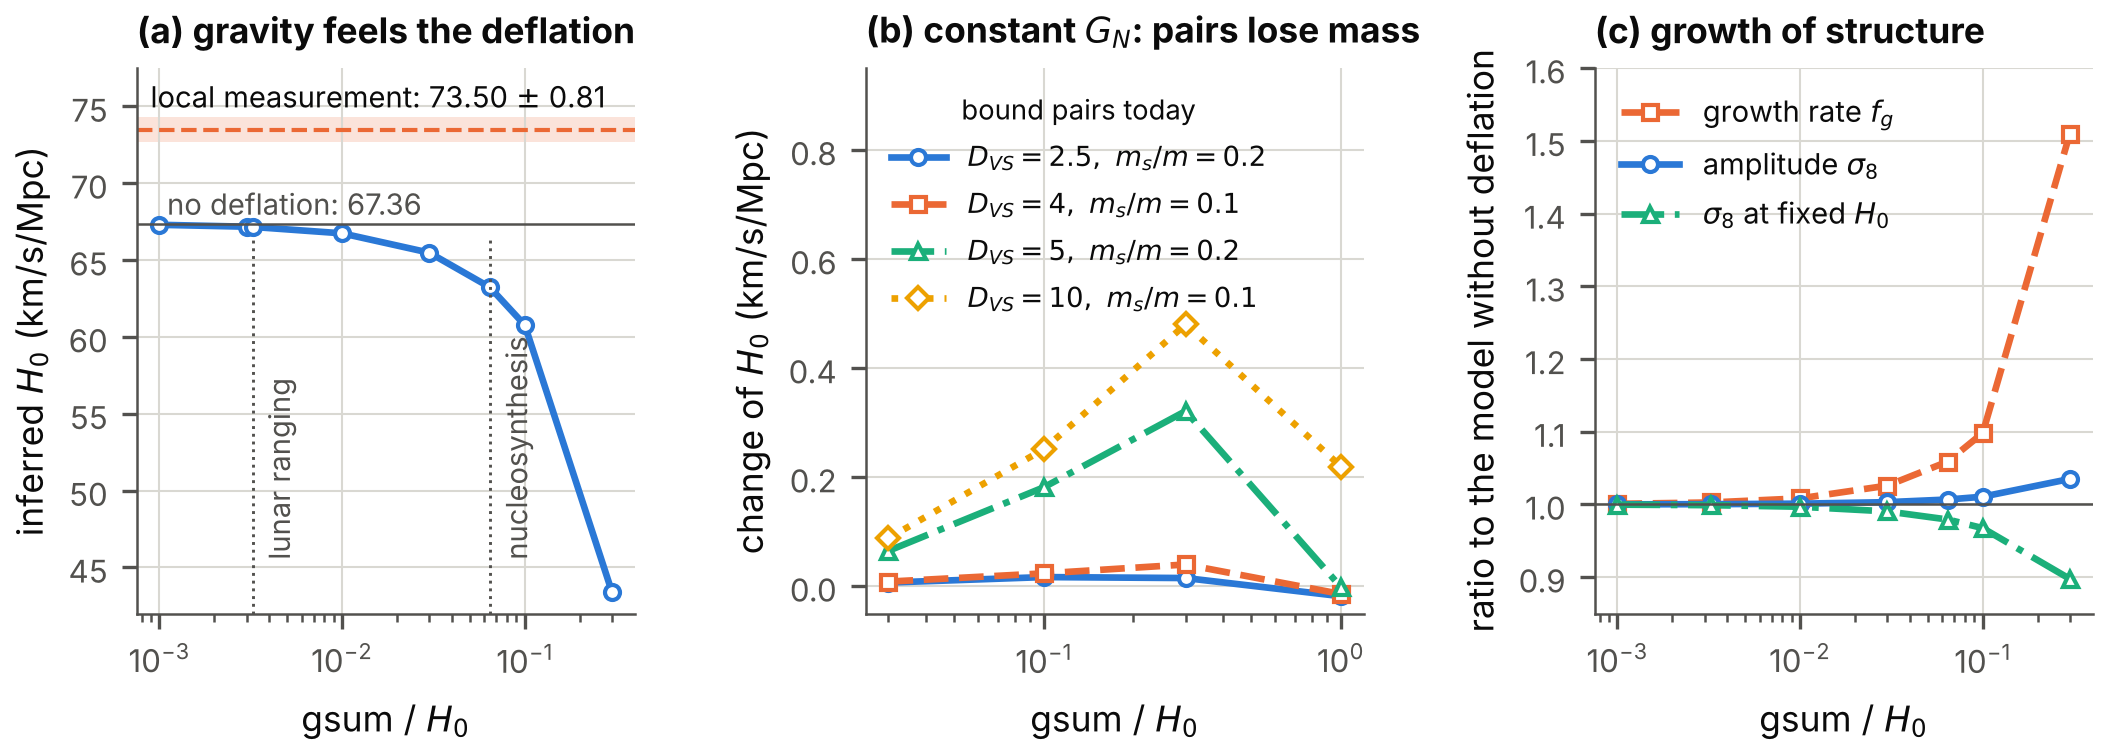
\includegraphics[width=1\textwidth,height=\textheight]{../figures/fig_hubble.png}
\caption{The Hubble constant and the growth of structure on a deflating
spacetime. (a) The Hubble constant inferred from the angular scale of
the sound horizon against the rate of deflation, if gravity feels the
deflation (A1, A2); the bounds of Sec. 3 are marked. (b) The change of
the inferred Hubble constant if Newton's constant is held fixed and
bound pairs lose rest mass (Sec. 4). (c) Amplitude and rate of the
growth of structure relative to the model without deflation (Sec. 5).
Data: \texttt{data/hubble\_deflation.csv},
\texttt{data/hubble\_mass\_loss.csv},
\texttt{data/growth\_deflation.csv}; programs:
\texttt{deflation\ cosmology}, \texttt{deflation\ matter}.}
\end{figure}

\begin{center}\rule{0.5\linewidth}{0.5pt}\end{center}

\hypertarget{how-fast-can-the-coordinates-deflate-today}{%
\section{3. How fast can the coordinates deflate
today?}\label{how-fast-can-the-coordinates-deflate-today}}

\begin{longtable}[]{@{}
  >{\raggedright\arraybackslash}p{(\columnwidth - 8\tabcolsep) * \real{0.1176}}
  >{\raggedright\arraybackslash}p{(\columnwidth - 8\tabcolsep) * \real{0.3235}}
  >{\raggedleft\arraybackslash}p{(\columnwidth - 8\tabcolsep) * \real{0.1176}}
  >{\raggedleft\arraybackslash}p{(\columnwidth - 8\tabcolsep) * \real{0.1176}}
  >{\raggedright\arraybackslash}p{(\columnwidth - 8\tabcolsep) * \real{0.3235}}@{}}
\toprule\noalign{}
\begin{minipage}[b]{\linewidth}\raggedright
observation
\end{minipage} & \begin{minipage}[b]{\linewidth}\raggedright
measured
\end{minipage} & \begin{minipage}[b]{\linewidth}\raggedleft
bound on gsum (per year)
\end{minipage} & \begin{minipage}[b]{\linewidth}\raggedleft
bound in units of \(H_0\)
\end{minipage} & \begin{minipage}[b]{\linewidth}\raggedright
assumption
\end{minipage} \\
\midrule\noalign{}
\endhead
\bottomrule\noalign{}
\endlastfoot
lunar laser ranging & \((dG_N/dt)/G_N\) = (7.1 \(\pm\) 7.6)
\(\times10^{-14}\) per year (68\%) & \(2.230\times10^{-13}\) &
\(3.237\times10^{-3}\) & gravity is eight-dimensional (A2) \\
primordial nucleosynthesis & \(G_N\)(nucleosynthesis)\(/G_N\)(today) =
0.99 +0.06 -0.05 (two sigma) & \(4.434\times10^{-12}\) & 0.0644 & A2,
and a rate that is constant from nucleosynthesis until today \\
primordial nucleosynthesis, weak interaction & \(G_{\rm Fermi}\) at
\(t=1\) s within 20 per cent (10 per cent) of today's value, fermion
masses held fixed & \(1.615\times10^{-11}\) (\(7.627\times10^{-12}\)) &
0.234 (0.111) & the assumption HV: the four-dimensional vacuum value of
the Vorton-Scalar sets the electroweak scale, as that of the Higgs field
does (not the author's hypothesis H2, in which the Higgs field is the
pair condensate); a rate that is constant from nucleosynthesis until
today; no assumption about gravity \\
atomic clocks, mass ratio & (d mu\_pe/dt)/mu\_pe = (-8 \(\pm\) 36)
\(\times10^{-18}\) per year (68\%), mu\_pe = ratio of the proton mass to
the electron mass & \(8.000\times10^{-17}\) & \(1.161\times10^{-6}\) &
the author's hypothesis H2 (the superfluid state is the Higgs field),
for n\_EW = 1; the bound scales as 1/n\_EW
(data/higgs\_scale\_exponent.csv) \\
atomic clocks & \((d\alpha_{\rm em}/dt)/\alpha_{\rm em}\) = (1.0 \(\pm\)
1.1) \(\times10^{-18}\) per year (68\%), \(\alpha_{\rm em}\) =
fine-structure constant & \(3.200\times10^{-18}\) &
\(4.645\times10^{-8}\) & an assumption outside the model, which contains
no electromagnetic field: stated to show how strongly such an extension
would be constrained \\
\end{longtable}

(The bound in units of \(H_0\) uses \(H_0=67.36\) km/s/Mpc. Sources:
lunar laser ranging, Ref. {[}1{]}; nucleosynthesis and Newton's
constant, Ref. {[}2{]}; nucleosynthesis and the Fermi constant, Ref.
{[}4{]}; atomic clocks, Ref. {[}3{]}.)

\begin{enumerate}
\def\labelenumi{\arabic{enumi}.}
\tightlist
\item
  \textbf{Under A2, lunar laser ranging} measures \((dG_N/dt)/G_N\)
  directly, and Eq. (1.1) turns its two-sigma limit into
  \(\mathrm{gsum}<2.23\times10^{-13}\) per year, that is
  \(3.24\times10^{-3}\,H_0\) (check \texttt{def-C3}). At this rate the
  deflation clock has advanced by
  \(\mathrm{gsum}\,t_0=3.1\times10^{-3}\) over the age \(t_0\) of the
  universe.
\item
  \textbf{Under A2, nucleosynthesis} bounds the ratio of Newton's
  constant then to its value today; for a rate that was constant since,
  \(\mathrm{gsum}<0.064\,H_0\). This is weaker than the first bound but
  does not assume that the rate today equals the rate in the past.
\item
  \textbf{Under HV, nucleosynthesis} bounds the change of the Fermi
  constant at fixed fermion masses to 10 to 20 per cent (Ref. {[}4{]}),
  which gives \(\mathrm{gsum}<0.111\) to \(0.234\,H_0\) (check
  \texttt{def-C5}). This bound does not involve gravity.
\item
  \textbf{Under the author's hypothesis H2, atomic clocks} give by far
  the strongest bound. The clocks compare transitions whose frequencies
  depend differently on the ratio \(m_p/m_e\) of the proton mass to the
  electron mass, and find it constant to \(8.0\times10^{-17}\) per year
  at two sigma (Ref. {[}3{]}). Under H2 the electron mass follows the
  electroweak scale and changes at the rate
  \(n_{\rm EW}\,\mathrm{gsum}\), while the proton mass, which is due
  mostly to the strong interaction, does not. Hence
  \[\mathrm{gsum}<\frac{8.0\times10^{-17}\ \text{per year}}{n_{\rm EW}}=\frac{1.16\times10^{-6}\,H_0}{n_{\rm EW}}\]
  (check \texttt{def-C6}). For \(n_{\rm EW}=1\) this is 2787 times
  stronger than the bound of lunar laser ranging, and it needs no
  assumption about gravity. The exponent \(n_{\rm EW}\) is of order one
  or larger wherever it has been computed (RS2, Sec. 5).
\item
  \textbf{The fine-structure constant} \(\alpha_{\rm em}\) is bounded by
  the same clocks to parts in \(10^{18}\) per year. This would bound the
  rate, to \(4.6\times10^{-8}\,H_0\), only if the electromagnetic field
  propagated along the deflating coordinates. The model contains no
  electromagnetic field; the row is included to show how strongly such
  an extension would be constrained.
\item
  \textbf{In the model as it stands} --- without H2, HV or an
  electromagnetic extension --- no mass and no coupling of ordinary
  matter depends on the deflation, and the atomic clocks do not bound
  the rate at all.
\end{enumerate}

\emph{Two corrections, recorded.} An earlier version of this table
derived a bound from the mass ratio by assuming that the electron mass
follows the four-dimensional vacuum value of the Vorton-Scalar. That was
an error: under HV the mass is the product of a coupling that grows and
a vacuum value that falls, and is constant (provenance RP9, item R-E7).
The same version attached the label H2 to the assumption HV; H2 is the
author's hypothesis about the pair condensate, and its consequence is
item 4 (RP9, item R-E23).

\textbf{The consequence for the histories of RS1 and RS4.} Under A2 the
clock has advanced by at most 0.0031 during the whole of cosmic history,
if the rate was constant; under H2 by at most
\(1.1\times10^{-6}/n_{\rm EW}\). The table of Sec. 6.3 shows what that
means quantity by quantity; in short, \emph{nothing happens}. A history
in which pairs become bound, matter becomes abnormal or the gap grows by
orders of magnitude within the age of the universe requires that gravity
does not feel the deflation (A2 abandoned), that the superfluid is not
the Higgs field (H2 abandoned), or that the rate was much larger in the
past than it is today.

\begin{figure}
\centering
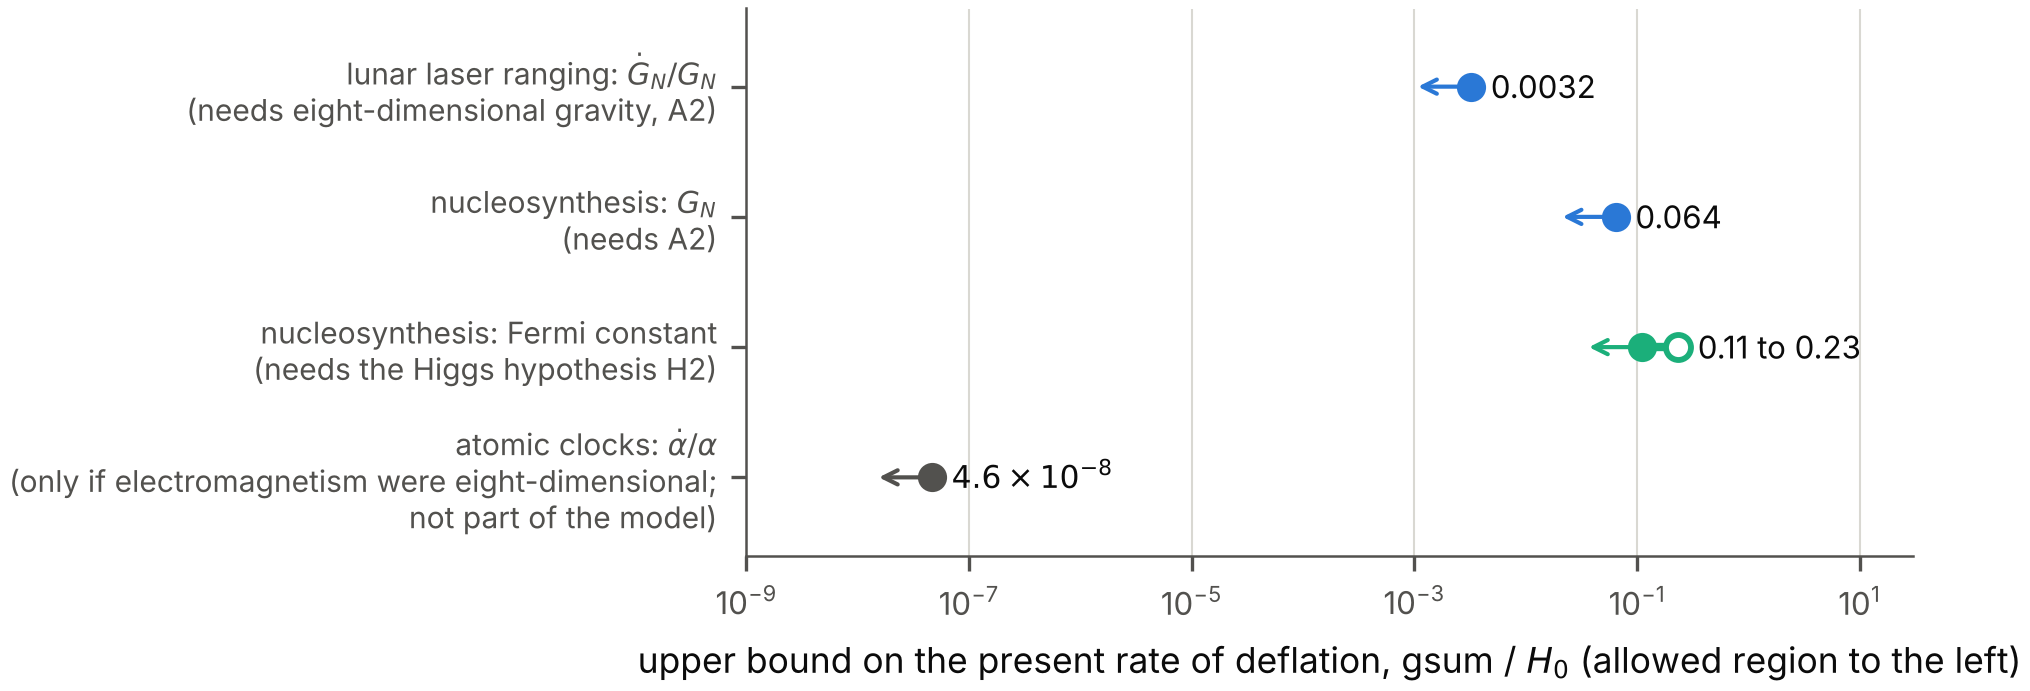
\includegraphics[width=1\textwidth,height=\textheight]{../figures/fig_bounds.png}
\caption{Upper bounds on the present total rate of deflation in units of
the Hubble constant, each under the assumption stated in the table of
this section. The allowed region is to the left of each bound. Data:
\texttt{data/deflation\_bounds.csv}; program:
\texttt{deflation\ cosmology}.}
\end{figure}

\begin{center}\rule{0.5\linewidth}{0.5pt}\end{center}

\hypertarget{bound-pairs-lose-rest-mass}{%
\section{4. Bound pairs lose rest
mass}\label{bound-pairs-lose-rest-mass}}

If the dark matter consists of bound pairs of the fermions, its
particles have the rest mass \(2m\) minus the binding energy. The
binding energy grows with the coupling (RS1, Sec. 4), so the pairs
become lighter as the deflation proceeds: the density of dark matter
falls slightly faster than the inverse volume. A dark matter that was
heavier in the past raises the inferred Hubble constant. The program
computes the effect for four examples with \(\alpha_{VS}\) between 0.4
and 1 today, where the binding energy is at most 8.2 per cent of the
rest mass (check \texttt{def-C4}):

\begin{longtable}[]{@{}
  >{\raggedleft\arraybackslash}p{(\columnwidth - 14\tabcolsep) * \real{0.1250}}
  >{\raggedleft\arraybackslash}p{(\columnwidth - 14\tabcolsep) * \real{0.1250}}
  >{\raggedleft\arraybackslash}p{(\columnwidth - 14\tabcolsep) * \real{0.1250}}
  >{\raggedleft\arraybackslash}p{(\columnwidth - 14\tabcolsep) * \real{0.1250}}
  >{\raggedleft\arraybackslash}p{(\columnwidth - 14\tabcolsep) * \real{0.1250}}
  >{\raggedleft\arraybackslash}p{(\columnwidth - 14\tabcolsep) * \real{0.1250}}
  >{\raggedleft\arraybackslash}p{(\columnwidth - 14\tabcolsep) * \real{0.1250}}
  >{\raggedleft\arraybackslash}p{(\columnwidth - 14\tabcolsep) * \real{0.1250}}@{}}
\toprule\noalign{}
\begin{minipage}[b]{\linewidth}\raggedleft
\(D_{VS}\) today
\end{minipage} & \begin{minipage}[b]{\linewidth}\raggedleft
\(m_s/m\)
\end{minipage} & \begin{minipage}[b]{\linewidth}\raggedleft
\(\alpha_{VS}\) today
\end{minipage} & \begin{minipage}[b]{\linewidth}\raggedleft
\(\mathrm{gsum}/H_0\)
\end{minipage} & \begin{minipage}[b]{\linewidth}\raggedleft
gravity feels the deflation
\end{minipage} & \begin{minipage}[b]{\linewidth}\raggedleft
mass today / early
\end{minipage} & \begin{minipage}[b]{\linewidth}\raggedleft
\(H_0\)
\end{minipage} & \begin{minipage}[b]{\linewidth}\raggedleft
change
\end{minipage} \\
\midrule\noalign{}
\endhead
\bottomrule\noalign{}
\endlastfoot
2.50 & 0.20 & 0.50 & 0.00324 & yes & 0.99995 & 67.16 & -0.20 \\
2.50 & 0.20 & 0.50 & 0.0644 & yes & 0.99905 & 63.25 & -4.11 \\
2.50 & 0.20 & 0.50 & 0.0300 & no & 0.99953 & 67.37 & 0.01 \\
2.50 & 0.20 & 0.50 & 0.100 & no & 0.99865 & 67.38 & 0.02 \\
2.50 & 0.20 & 0.50 & 0.300 & no & 0.99736 & 67.38 & 0.02 \\
2.50 & 0.20 & 0.50 & 1.00 & no & 0.99721 & 67.34 & -0.02 \\
5.00 & 0.20 & 1.00 & 0.00324 & yes & 0.99950 & 67.17 & -0.19 \\
5.00 & 0.20 & 1.00 & 0.0644 & yes & 0.99085 & 63.36 & -4.00 \\
5.00 & 0.20 & 1.00 & 0.0300 & no & 0.99557 & 67.42 & 0.06 \\
5.00 & 0.20 & 1.00 & 0.100 & no & 0.98658 & 67.54 & 0.18 \\
5.00 & 0.20 & 1.00 & 0.300 & no & 0.96882 & 67.68 & 0.32 \\
5.00 & 0.20 & 1.00 & 1.00 & no & 0.95069 & 67.36 & 0.00 \\
4.00 & 0.10 & 0.40 & 0.00324 & yes & 0.99994 & 67.16 & -0.20 \\
4.00 & 0.10 & 0.40 & 0.0644 & yes & 0.99880 & 63.25 & -4.11 \\
4.00 & 0.10 & 0.40 & 0.0300 & no & 0.99942 & 67.37 & 0.01 \\
4.00 & 0.10 & 0.40 & 0.100 & no & 0.99824 & 67.38 & 0.02 \\
4.00 & 0.10 & 0.40 & 0.300 & no & 0.99594 & 67.40 & 0.04 \\
4.00 & 0.10 & 0.40 & 1.00 & no & 0.99408 & 67.35 & -0.01 \\
10.00 & 0.10 & 1.00 & 0.00324 & yes & 0.99933 & 67.17 & -0.19 \\
10.00 & 0.10 & 1.00 & 0.0644 & yes & 0.98756 & 63.40 & -3.96 \\
10.00 & 0.10 & 1.00 & 0.0300 & no & 0.99400 & 67.45 & 0.09 \\
10.00 & 0.10 & 1.00 & 0.100 & no & 0.98168 & 67.61 & 0.25 \\
10.00 & 0.10 & 1.00 & 0.300 & no & 0.95635 & 67.84 & 0.48 \\
10.00 & 0.10 & 1.00 & 1.00 & no & 0.92342 & 67.58 & 0.22 \\
\end{longtable}

\begin{itemize}
\tightlist
\item
  \emph{If gravity feels the deflation} (rows ``yes''), the inferred
  Hubble constant changes by between \(-4.11\) and \(-0.19\) km/s/Mpc at
  the rates that nucleosynthesis and lunar laser ranging allow: the
  weaker gravity of the past outweighs the loss of mass.
\item
  \emph{If Newton's constant is held fixed} and the deflation acts on
  the dark sector alone (rows ``no''), rates between 0.03 and \(1\,H_0\)
  raise the inferred Hubble constant by at most \(+0.48\) km/s/Mpc, for
  a loss of up to 7.7 per cent of the rest mass.
\end{itemize}

The loss of rest mass is the only effect of the deflation found here
that raises the inferred Hubble constant. In these examples it supplies
less than a tenth of the 6.1 km/s/Mpc that separate 67.36 from the local
value.

\begin{center}\rule{0.5\linewidth}{0.5pt}\end{center}

\hypertarget{the-growth-of-structure}{%
\section{5. The growth of structure}\label{the-growth-of-structure}}

Under A1 and A2 the density contrast \(\delta_m\) of matter in ordinary
space obeys, in the Newtonian limit, the usual equation with the
Newton's constant of the moment,
\[\frac{d^2\delta_m}{dx4^2}+2H\,\frac{d\delta_m}{dx4}=4\pi\,G_N(x4)\,\rho_m\,\delta_m .\]
The program integrates it for each model of Sec. 2 and reports the
amplitude today relative to the model without deflation --- the ratio of
the amplitudes \(\sigma_8\) for the same primordial amplitude --- and
the growth rate \(f_g=d\ln\delta_m/d\ln a_{\rm sp}\) today (check
\texttt{def-D4}):

\begin{longtable}[]{@{}
  >{\raggedleft\arraybackslash}p{(\columnwidth - 12\tabcolsep) * \real{0.1429}}
  >{\raggedleft\arraybackslash}p{(\columnwidth - 12\tabcolsep) * \real{0.1429}}
  >{\raggedleft\arraybackslash}p{(\columnwidth - 12\tabcolsep) * \real{0.1429}}
  >{\raggedleft\arraybackslash}p{(\columnwidth - 12\tabcolsep) * \real{0.1429}}
  >{\raggedleft\arraybackslash}p{(\columnwidth - 12\tabcolsep) * \real{0.1429}}
  >{\raggedleft\arraybackslash}p{(\columnwidth - 12\tabcolsep) * \real{0.1429}}
  >{\raggedleft\arraybackslash}p{(\columnwidth - 12\tabcolsep) * \real{0.1429}}@{}}
\toprule\noalign{}
\begin{minipage}[b]{\linewidth}\raggedleft
\(\mathrm{gsum}/H_0\)
\end{minipage} & \begin{minipage}[b]{\linewidth}\raggedleft
\(H_0\)
\end{minipage} & \begin{minipage}[b]{\linewidth}\raggedleft
\(\sigma_8\) ratio
\end{minipage} & \begin{minipage}[b]{\linewidth}\raggedleft
\(f_g\) ratio
\end{minipage} & \begin{minipage}[b]{\linewidth}\raggedleft
\(f_g\sigma_8\) ratio
\end{minipage} & \begin{minipage}[b]{\linewidth}\raggedleft
\(\sigma_8\) ratio, fixed \(H_0\)
\end{minipage} & \begin{minipage}[b]{\linewidth}\raggedleft
\(f_g\) ratio, fixed \(H_0\)
\end{minipage} \\
\midrule\noalign{}
\endhead
\bottomrule\noalign{}
\endlastfoot
0 & 67.36 & 1.0000 & 1.0000 & 1.0000 & 1.0000 & 1.0000 \\
0.00100 & 67.30 & 1.0001 & 1.0008 & 1.0009 & 0.9997 & 0.9998 \\
0.00324 & 67.16 & 1.0003 & 1.0027 & 1.0030 & 0.9990 & 0.9993 \\
0.0100 & 66.74 & 1.0010 & 1.0083 & 1.0093 & 0.9968 & 0.9979 \\
0.0300 & 65.48 & 1.0031 & 1.0258 & 1.0290 & 0.9904 & 0.9937 \\
0.0644 & 63.23 & 1.0067 & 1.0589 & 1.0661 & 0.9792 & 0.9865 \\
0.100 & 60.77 & 1.0106 & 1.0982 & 1.1098 & 0.9674 & 0.9790 \\
0.300 & 43.41 & 1.0350 & 1.5100 & 1.5628 & 0.8975 & 0.9365 \\
\end{longtable}

Two effects oppose each other. At a \emph{fixed} Hubble constant, weaker
gravity in the past lowers the amplitude:
\(d\ln\sigma_8/d(\mathrm{gsum}/H_0)=-0.317\). But the Hubble constant
that keeps the sound-horizon angle is lower, the cosmological term takes
over later, and matter clusters for longer; with that Hubble constant
the net change is \(+0.102\) per unit of \(\mathrm{gsum}/H_0\). The
amplitude therefore barely moves --- \(+0.03\) per cent at the bound of
lunar laser ranging, \(+0.67\) per cent at the bound of nucleosynthesis
--- while the growth rate today rises by the factors 1.0027 and 1.0589.
A deflating universe would show itself in the product \(f_g\sigma_8\),
which redshift-space distortions measure, rather than in \(\sigma_8\).

\begin{center}\rule{0.5\linewidth}{0.5pt}\end{center}

\hypertarget{dark-matter}{%
\section{6. Dark matter}\label{dark-matter}}

\hypertarget{what-does-not-change}{%
\subsection{6.1 What does not change}\label{what-does-not-change}}

The estimates of S3 that decide whether the particles of the model can
be degenerate or condensed in observed halos contain the masses, the
densities and the velocities only. The masses do not change along the
deflation. Computed again, every number agrees with the main project:
fermions with eight internal states are degenerate in the core of a
dwarf galaxy only if lighter than 0.276 keV, and bound pairs are
condensed there only if lighter than 262 eV (check \texttt{def-D1}). The
verdict of S3 on these two possibilities stands.

\hypertarget{self-interaction-and-the-epoch-of-the-resonance}{%
\subsection{6.2 Self-interaction, and the epoch of the
resonance}\label{self-interaction-and-the-epoch-of-the-resonance}}

\emph{Bound pairs.} S3 requires the cross-section per mass of the pairs,
\(8\pi/m_s^2\) divided by the pair mass, to respect the bound of about 1
cm\(^2\)/g from colliding clusters, and derives the smallest allowed
fermion mass: 918 MeV for \(\alpha_{VS}=0.1\). For a given particle the
masses are constant and so is this cross-section; what the deflation
changes is whether the pair \emph{exists}: it is bound only after
\(D_{VS}\) has grown to 1.67981. In terms of the coupling of the moment
the smallest mass falls as \(\alpha_{VS}^{-2/3}\), that is as
\(e^{-2\tau_d/3}\) (check \texttt{def-D2}).

\emph{The moment of binding.} By RS1, Sec. 4.1, the scattering length of
two unbound fermions diverges when \(D_{VS}\) passes \(D_c\). The
cross-section then rises to the limit that unitarity allows, which is
larger the slower the particles. For the example particle of S3
(\(m=918\) MeV, \(m_s=54.7\) MeV) and the relative velocities 10, 156
and 1000 km/s (check \texttt{def-D3}):

\begin{itemize}
\tightlist
\item
  one unit of the clock before the binding the cross-section per mass is
  0.84 cm\(^2\)/g at all three velocities;
\item
  at the binding it peaks at \(1.3\times10^{7}\), \(5.2\times10^{4}\)
  and \(1.3\times10^{3}\) cm\(^2\)/g;
\item
  it exceeds 100 cm\(^2\)/g during an interval of the clock of 0.268,
  0.268 and 0.258 around the binding.
\end{itemize}

\textbf{A deflating universe whose dark matter consists of these
fermions passes through an epoch of strong, velocity-dependent
self-interaction} --- strongest in the smallest halos. Panel (c) of the
figure in RS1, Sec. 4.1, shows the three curves. Whether the epoch lies
in the observable past depends on the rate: by Sec. 3, under A2 and a
constant rate it does so only if \(D_{VS}\) today exceeds \(D_c\) by
less than a third of a per cent, a coincidence that nothing in the model
explains.

\hypertarget{how-fast-the-quantities-drift}{%
\subsection{6.3 How fast the quantities
drift}\label{how-fast-the-quantities-drift}}

With \(n=d\ln(\text{quantity})/d\tau_d\), the relative change of a
quantity over the age of the universe is \(n\,\mathrm{gsum}\,t_0\)
(\(H_0t_0=0.9516\) for the model without deflation; check
\texttt{def-D5}):

\begin{longtable}[]{@{}
  >{\raggedright\arraybackslash}p{(\columnwidth - 10\tabcolsep) * \real{0.1667}}
  >{\raggedright\arraybackslash}p{(\columnwidth - 10\tabcolsep) * \real{0.1667}}
  >{\raggedleft\arraybackslash}p{(\columnwidth - 10\tabcolsep) * \real{0.1667}}
  >{\raggedleft\arraybackslash}p{(\columnwidth - 10\tabcolsep) * \real{0.1667}}
  >{\raggedleft\arraybackslash}p{(\columnwidth - 10\tabcolsep) * \real{0.1667}}
  >{\raggedleft\arraybackslash}p{(\columnwidth - 10\tabcolsep) * \real{0.1667}}@{}}
\toprule\noalign{}
\begin{minipage}[b]{\linewidth}\raggedright
quantity
\end{minipage} & \begin{minipage}[b]{\linewidth}\raggedright
where evaluated
\end{minipage} & \begin{minipage}[b]{\linewidth}\raggedleft
\(n\)
\end{minipage} & \begin{minipage}[b]{\linewidth}\raggedleft
change at the bound of lunar laser ranging
\end{minipage} & \begin{minipage}[b]{\linewidth}\raggedleft
at the bound of nucleosynthesis (\(G_N\))
\end{minipage} & \begin{minipage}[b]{\linewidth}\raggedleft
at the bound of nucleosynthesis (\(G_{\rm Fermi}\))
\end{minipage} \\
\midrule\noalign{}
\endhead
\bottomrule\noalign{}
\endlastfoot
\(\alpha_{VS}\), \(G_{VS}\), \(D_{VS}\), \(C\) & any & 1.000 &
\(3.08\times10^{-3}\) & 0.0612 & 0.223 \\
\(g_{VS}\) & any & 0.500 & \(1.54\times10^{-3}\) & 0.0306 & 0.112 \\
fermion mass \(m\), mass \(m_s\) of the radial mode & any & 0.000 & 0 &
0 & 0 \\
scattering length of two fermions (no bound state) & \(D_{VS}\) = 0.5 &
1.368 & \(4.21\times10^{-3}\) & 0.0838 & 0.305 \\
scattering length of two fermions (no bound state) & \(D_{VS}\) = 1 &
2.336 & \(7.20\times10^{-3}\) & 0.143 & 0.521 \\
scattering length of two fermions (no bound state) & \(D_{VS}\) = 1.5 &
9.092 & 0.0280 & 0.557 & 2.03 \\
binding energy of the pair & \(D_{VS}\) = 1.8 & 30.129 & 0.0928 & 1.85 &
6.72 \\
binding energy of the pair & \(D_{VS}\) = 2 & 12.657 & 0.0390 & 0.775 &
2.82 \\
binding energy of the pair & \(D_{VS}\) = 3 & 4.673 & 0.0144 & 0.286 &
1.04 \\
binding energy of the pair & \(D_{VS}\) = 5 & 3.101 &
\(9.55\times10^{-3}\) & 0.190 & 0.692 \\
binding energy of the pair & \(D_{VS}\) = 10 & 2.456 &
\(7.57\times10^{-3}\) & 0.150 & 0.548 \\
rest mass of the bound pair & \(D_{VS}\) = 5, \(m_s/m\) = 0.2 & -0.162 &
\(-4.99\times10^{-4}\) & \(-9.91\times10^{-3}\) & -0.0361 \\
rest mass of the bound pair & \(D_{VS}\) = 10, \(m_s/m\) = 0.1 & -0.218
& \(-6.73\times10^{-4}\) & -0.0134 & -0.0488 \\
gap and critical temperature of the paired state (weak coupling) &
pairing strength \(\lambda\) = 0.15 & 6.667 & 0.0205 & 0.408 & 1.49 \\
gap and critical temperature of the paired state (weak coupling) &
pairing strength \(\lambda\) = 0.2 & 5.000 & 0.0154 & 0.306 & 1.12 \\
gap and critical temperature of the paired state (weak coupling) &
pairing strength \(\lambda\) = 0.3 & 3.333 & 0.0103 & 0.204 & 0.744 \\
cross-section of two fermions at low energy (Born regime,
\(D_{VS}\ll1\)) & \(D_{VS}\) = 0.05 & 2.052 & \(6.32\times10^{-3}\) &
0.126 & 0.458 \\
\end{longtable}

The couplings themselves drift with \(n=1\) or \(\tfrac12\). Quantities
near a threshold drift much faster: the scattering length just below the
binding with \(n=9.1\), the binding energy just above it with \(n=30\),
the gap of a weakly paired state with \(n=1/\lambda\). These are the
quantities in which a slow deflation would first be seen.

\begin{center}\rule{0.5\linewidth}{0.5pt}\end{center}

\hypertarget{the-quanta-that-the-deflation-creates}{%
\section{7. The quanta that the deflation
creates}\label{the-quanta-that-the-deflation-creates}}

On the 7+1 spacetime the deflation creates quanta in modes that depend
on a deflating coordinate, with the thermal spectrum of the temperature
\(T_{\rm defl}=\hbar\,\mathrm{rate}_t/2\pi k_B\) (DMD, Sec. 4.2; RS1,
Sec. 2.3). For three equal rates at the largest total rates that the
bounds allow (check \texttt{def-D6}):

\begin{longtable}[]{@{}
  >{\raggedright\arraybackslash}p{(\columnwidth - 10\tabcolsep) * \real{0.1667}}
  >{\raggedleft\arraybackslash}p{(\columnwidth - 10\tabcolsep) * \real{0.1667}}
  >{\raggedleft\arraybackslash}p{(\columnwidth - 10\tabcolsep) * \real{0.1667}}
  >{\raggedleft\arraybackslash}p{(\columnwidth - 10\tabcolsep) * \real{0.1667}}
  >{\raggedleft\arraybackslash}p{(\columnwidth - 10\tabcolsep) * \real{0.1667}}
  >{\raggedleft\arraybackslash}p{(\columnwidth - 10\tabcolsep) * \real{0.1667}}@{}}
\toprule\noalign{}
\begin{minipage}[b]{\linewidth}\raggedright
bound
\end{minipage} & \begin{minipage}[b]{\linewidth}\raggedleft
\(\mathrm{gsum}/H_0\)
\end{minipage} & \begin{minipage}[b]{\linewidth}\raggedleft
\(\hbar\,\mathrm{rate}_t\) (eV)
\end{minipage} & \begin{minipage}[b]{\linewidth}\raggedleft
\(T_{\rm defl}\) (K)
\end{minipage} & \begin{minipage}[b]{\linewidth}\raggedleft
exponent for \(m=1\) keV
\end{minipage} & \begin{minipage}[b]{\linewidth}\raggedleft
exponent for \(m=1\) GeV
\end{minipage} \\
\midrule\noalign{}
\endhead
\bottomrule\noalign{}
\endlastfoot
lunar laser ranging (A2) & 0.00324 & \(1.55\times10^{-36}\) &
\(2.86\times10^{-33}\) & \(4.05\times10^{39}\) &
\(4.05\times10^{45}\) \\
nucleosynthesis, \(G_N\) (A2) & 0.0644 & \(3.08\times10^{-35}\) &
\(5.69\times10^{-32}\) & \(2.04\times10^{38}\) &
\(2.04\times10^{44}\) \\
nucleosynthesis, \(G_{\rm Fermi}\) (HV), 20 per cent & 0.234 &
\(1.12\times10^{-34}\) & \(2.07\times10^{-31}\) & \(5.59\times10^{37}\)
& \(5.59\times10^{43}\) \\
\(\mathrm{gsum}=H_0\) & 1.00 & \(4.79\times10^{-34}\) &
\(8.85\times10^{-31}\) & \(1.31\times10^{37}\) &
\(1.31\times10^{43}\) \\
\end{longtable}

The exponent is \(2\pi m/\mathrm{rate}_t\); the number of created
particles of mass \(m\) per mode is \(e^{-\text{exponent}}\). At any
rate allowed today the temperature is below \(10^{-30}\) K and the
exponent above \(10^{37}\) for every mass above 1 keV: \textbf{no
particle is created today.} Creation by deflation matters only for an
epoch in which the rate was comparable with the masses, which no bound
of Sec. 3 addresses.

\begin{center}\rule{0.5\linewidth}{0.5pt}\end{center}

\hypertarget{verdicts-on-the-two-hypotheses}{%
\section{8. Verdicts on the two
hypotheses}\label{verdicts-on-the-two-hypotheses}}

\textbf{The Hubble tension.} On the deflating spacetimes the mechanisms
of the main project (S3, Sec. 3: the phase mode of the Vorton-Scalar as
dark radiation) are untouched at the allowed rates, since the couplings
drift by parts in a thousand; their verdict in S3 stands and is not
improved. The deflation itself contributes two effects. The first,
through Newton's constant, has the wrong sign and is bounded to 0.2
km/s/Mpc. The second, the loss of mass of bound pairs, has the right
sign and is bounded, in the examples computed, to 0.5 km/s/Mpc.
\textbf{The hypothesis that the model resolves the Hubble tension is not
supported by the deflation, and under A2 it is mildly disfavoured.}

\textbf{The Higgs hypothesis and the deflation together.} If the
superfluid is the Higgs field (H2), the atomic clocks limit the rate of
deflation to \(1.16\times10^{-6}\,H_0/n_{\rm EW}\): the two hypotheses
can both hold only if the deflation is, for every purpose of this
supplement, switched off today.

\textbf{Dark matter.} The conclusions of S3 about the mass ranges hold
unchanged. The deflation adds one qualitative prediction, the resonance
epoch of Sec. 6.2, and one quantitative one, the shift of the growth
rate of Sec. 5. Neither is in conflict with observation at the allowed
rates, and neither is detectable at the rate that lunar laser ranging
allows. \textbf{The hypothesis that the superfluid is the dark matter is
neither strengthened nor weakened by the deflation}; it acquires a
history, whose observable part is empty if gravity is eight-dimensional
and the rate constant.

\begin{center}\rule{0.5\linewidth}{0.5pt}\end{center}

\hypertarget{what-has-been-established-and-what-has-not}{%
\section{9. What has been established, and what has
not}\label{what-has-been-established-and-what-has-not}}

\textbf{Established}, each under the assumptions named:

\begin{enumerate}
\def\labelenumi{\arabic{enumi}.}
\tightlist
\item
  the equation of the expansion (1.2) (A1, A2) and the fall of the
  inferred Hubble constant, \(d\ln H_0/d(\mathrm{gsum}/H_0)=-0.911\),
  verified by an independent integration;
\item
  the bounds of Sec. 3 on the present rate (under A2; under HV; under
  the author's hypothesis H2, from atomic clocks; under an
  electromagnetic extension), and that in the model as it stands the
  atomic clocks give none;
\item
  the effect of the loss of mass of bound pairs on the inferred Hubble
  constant (Sec. 4);
\item
  the growth of structure (A1, A2; Sec. 5);
\item
  the unchanged estimates of degeneracy and condensation, the resonance
  epoch, and the table of drifts (Sec. 6);
\item
  the temperature of the created quanta at the allowed rates (Sec. 7).
\end{enumerate}

\textbf{Not established.}

\begin{enumerate}
\def\labelenumi{\arabic{enumi}.}
\tightlist
\item
  \emph{The spectra of the microwave background.} S3 of the main project
  computes the temperature and polarization spectra with its own
  Einstein--Boltzmann program and forecasts the constraints from them.
  The revision has \textbf{not} repeated this calculation with a
  time-dependent Newton's constant, for two reasons. First, the
  equations of the perturbations contain the stresses of the source that
  keeps the rates of deflation constant, which the hypotheses do not
  specify (item 2 below): a spectrum can be computed only under a
  further assumption, which is the author's to make. Second, it requires
  a copy of that program in which the gravitational coupling of the
  background and of the perturbations depends on time while the rates of
  Thomson scattering and of recombination do not, validated again
  against the constant case; it cannot be emulated by changing
  parameters of the existing program. What Sec. 2 establishes is the
  effect on the \emph{background}. At the bound of lunar laser ranging
  Newton's constant at last scattering was 0.9969 of today's value; the
  effect on the spectra beyond the shift of the sound-horizon angle is
  of that relative size, and has not been computed. This item is
  recorded in the provenance RP0 as open, awaiting the author's
  instruction.
\item
  \emph{The other field equations, and the theory of gravity.} Only the
  time component (1.2) of Einstein's equations is used. The spatial
  components constrain the stresses of the source that drives the
  deflation, which is unknown. Whether a source exists that keeps three
  rates constant while ordinary space expands has not been examined.
  DMD, Sec. 1.4a, shows that \emph{without} expansion of ordinary space
  and with three equal rates the deflating spacetimes solve the
  equations of Einstein--Gauss--Bonnet gravity without any source. If
  gravity is of that kind, assumption A2 does not hold as stated: the
  relation (1.1) between Newton's constant and the volume of the
  deflating coordinates, and with it every bound and every result of
  this supplement that is marked A2, would have to be derived anew.
\item
  \emph{A varying rate.} All bounds that reach back to nucleosynthesis
  assume a constant rate. A rate that was large early and is small today
  is neither excluded nor described.
\item
  \emph{The dynamics of the resonance epoch.} Sec. 6.2 gives
  cross-sections; the consequences for the formation of halos during the
  epoch have not been simulated.
\item
  \emph{Extensions.} The bound from the fine-structure constant concerns
  a theory with an electromagnetic field in eight dimensions, which is
  not the model.
\end{enumerate}

\begin{center}\rule{0.5\linewidth}{0.5pt}\end{center}

\hypertarget{appendix-a.-complete-output-of-the-programs}{%
\section{Appendix A. Complete output of the
programs}\label{appendix-a.-complete-output-of-the-programs}}

\hypertarget{a.1-deflation-cosmology}{%
\subsection{\texorpdfstring{A.1
\texttt{deflation\ cosmology}}{A.1 deflation cosmology}}\label{a.1-deflation-cosmology}}

\begin{Shaded}
\begin{Highlighting}[]
\NormalTok{PROJECT spacetimes, Revision\_Deflation: checks of the cosmological calculations on the deflating spacetime}
\NormalTok{generated by: deflation (Rust crate spacetimes{-}deflation, version 0.1.0; PROJECT spacetimes, Revision\_Deflation); command: deflation cosmology}
\NormalTok{6 of 6 checks passed}

\NormalTok{[PASS] def{-}C1  (numerical) without deflation the background integrals of this module agree with the main project (its recombination calculation gives z\_* = 1089.92): 100 theta\_* = 1.03965 here against 1.03965, sound horizon 144.449 Mpc against 144.449 Mpc; age 13.814 Gyr}
\NormalTok{[PASS] def{-}C2  (numerical) with deflation at a constant rate, gravity was weaker in the past, the early universe expanded more slowly at a given density, and the sound horizon is larger; holding 100 theta\_*, omega\_b and omega\_c fixed, the inferred Hubble constant FALLS monotonically with the rate: d ln H\_0/d(gsum/H\_0) = {-}0.911 at small rates; H\_0 = 66.74, 65.48, 60.77 km/s/Mpc for gsum = 0.01, 0.03, 0.1 H\_0 (67.36 without deflation). Deflation moves the Hubble constant away from the locally measured value}
\NormalTok{[PASS] def{-}C3  (numerical) bounds on the present rate of deflation if gravity is eight{-}dimensional (G\_N grows at the rate gsum): lunar laser ranging, (dG\_N/dt)/G\_N = (7.1 +{-} 7.6) 10\^{}{-}14 per year, gives gsum \textless{} 2.23e{-}13 per year = 3.24e{-}3 H\_0 at two sigma; nucleosynthesis, G\_N(nucleosynthesis)/G\_N(today) \textgreater{} 0.94 at two sigma, gives gsum \textless{} 4.43e{-}12 per year = 0.064 H\_0 for a rate that was constant since then. At these rates the inferred Hubble constant changes by {-}0.199 and {-}4.13 km/s/Mpc: the local measurement, 73.50 +{-} 0.81 km/s/Mpc, cannot be approached. Over the age t\_0 of the model without deflation (H\_0 t\_0 = 0.9516) the deflation clock has advanced by gsum t\_0 = 3.1e{-}3 at the first of these rates}
\NormalTok{[PASS] def{-}C5  (numerical) bounds that do not rest on gravity: (i) under the assumption HV (the vacuum value of the Vorton{-}Scalar sets the electroweak scale) the Fermi constant grows at the rate gsum while every mass stays constant; nucleosynthesis with fixed masses allows G\_Fermi at t = 1 s to differ by 10 to 20 per cent from today\textquotesingle{}s value (Scherrer and Spergel 1993), which gives gsum \textless{} 0.111 to 0.234 H\_0, weaker than the bound from Newton\textquotesingle{}s constant; (ii) in the model as it stands (without H2 and without HV) no mass of ordinary matter depends on the deflation, and the measured constancy of the ratio of the proton mass to the electron mass does not bound the rate; (iii) the fine{-}structure constant would bound it, gsum \textless{} 3.2e{-}18 per year = 4.6e{-}8 H\_0, only if the electromagnetic field propagated along the deflating coordinates, which is not part of the model}
\NormalTok{[PASS] def{-}C6  (numerical) the author\textquotesingle{}s hypothesis H2 (the superfluid state is the Higgs field) on a deflating spacetime: the electroweak scale is then the scale of the pair condensate, which depends on alpha\_VS, and alpha\_VS grows as exp(gsum x4). With n\_EW = d ln v\_EW/d ln alpha\_VS the electron mass changes at the rate n\_EW gsum and the proton mass does not; atomic clocks (ratio of the two masses constant to 8.0e{-}17 per year at two sigma) then give gsum \textless{} 8.0e{-}17 per year / n\_EW = 1.16e{-}6 H\_0 / n\_EW, a bound 2787 times stronger than that of lunar laser ranging for n\_EW = 1, and one that needs no assumption about gravity; over the age of the universe the deflation clock can then have advanced by at most 1.1e{-}6/n\_EW. In the scale{-}invariant ladder equation of the main project n\_EW = (1 + 4 rho\_c\^{}2) atan(1/(2 rho\_c))/(8 rho\_c\^{}3) + 1/(4 rho\_c\^{}2) with rho\_c\^{}2 = (alpha\_VS/alpha\_c {-} 1)/4 (agreement with the numerical derivative: 2.8e{-}8): n\_EW = 15.1, 2.57, 1.15, 0.54 for alpha\_VS/alpha\_c = 1.25, 2, 3, 5; it diverges at the critical coupling and exceeds 1 for alpha\_VS \textless{} 3.27 alpha\_c. For the model itself (massive fermions, massive radial mode) n\_EW has not been computed}
\NormalTok{[PASS] def{-}C4  (numerical) dark matter of bound pairs loses rest mass while the coupling grows, because the binding energy increases (four examples with alpha\_VS = 0.4 to 1 today; binding energy at most 8.2 per cent of the rest mass). If gravity feels the deflation, the inferred Hubble constant changes by between {-}4.11 and {-}0.19 km/s/Mpc at the rates that lunar laser ranging and nucleosynthesis allow: it falls, the weaker gravity of the past outweighing the loss of mass. If Newton\textquotesingle{}s constant is held fixed and the deflation acts on the dark sector alone, rates between 0.03 and 1 H\_0 change the inferred Hubble constant by at most +0.48 km/s/Mpc, for a loss of up to 7.7 per cent of the rest mass (data/hubble\_mass\_loss.csv). The loss of rest mass is the only effect of the deflation that raises the inferred Hubble constant; in these examples it supplies less than a tenth of the 6.1 km/s/Mpc that separate 67.36 from the local value 73.50}
\NormalTok{[PASS] ALL  (numerical) every check above passed}
\end{Highlighting}
\end{Shaded}

\hypertarget{a.2-deflation-matter}{%
\subsection{\texorpdfstring{A.2
\texttt{deflation\ matter}}{A.2 deflation matter}}\label{a.2-deflation-matter}}

\begin{Shaded}
\begin{Highlighting}[]
\NormalTok{PROJECT spacetimes, Revision\_Deflation: checks of the dark{-}matter estimates on the deflating spacetime}
\NormalTok{generated by: deflation (Rust crate spacetimes{-}deflation, version 0.1.0; PROJECT spacetimes, Revision\_Deflation); command: deflation matter}
\NormalTok{6 of 6 checks passed}

\NormalTok{[PASS] def{-}D1  (numerical) the estimates of degeneracy and of condensation in halos contain no coupling: fermions with eight internal states are degenerate in the core of a dwarf galaxy only below 0.276 keV, bound pairs are condensed there only below 262 eV. Computed again; every number agrees with the file of the main project (the masses do not change along the deflation)}
\NormalTok{[PASS] def{-}D2  (numerical) self{-}interaction of bound pairs: with the coupling of today the table of the main project is reproduced (smallest fermion mass 918 MeV for alpha\_VS = 0.1). The smallest mass falls as alpha\_VS\^{}({-}2/3), that is, as exp({-}2 tau\_d/3) along the deflation. For a given particle the masses m and m\_s are constant, hence so is the cross{-}section 8 pi/m\_s\^{}2 of the pairs; the deflation changes whether the pair exists: it is bound only after D\_VS = alpha\_VS m/m\_s has grown to 1.67981}
\NormalTok{[PASS] def{-}D3  (numerical) the moment at which the pair becomes bound is a zero{-}energy resonance of the scattering of two fermions: the scattering length diverges at D\_VS = D\_c. For a particle with m = 918 MeV and m\_s = 54.7 MeV the cross{-}section per mass at the relative velocities 10, 156 and 1000 km/s rises from 8.4e{-}1, 8.4e{-}1, 8.4e{-}1 cm\^{}2/g one unit of the deflation clock before the binding to the peak values 1.3e7, 5.2e4, 1.3e3 cm\^{}2/g (limit of unitarity at 10 km/s: 1.3e7); it exceeds 100 cm\^{}2/g during an interval of the clock of 0.268, 0.268, 0.258 around the moment of binding. A deflating universe in which the dark matter is made of these fermions passes through an epoch of strong, velocity{-}dependent self{-}interaction}
\NormalTok{[PASS] def{-}D4  (numerical) growth of structure when Newton\textquotesingle{}s constant grows with the deflation (A1, A2). Two effects oppose each other. (i) Gravity was weaker in the past: at a fixed Hubble constant the amplitude today (sigma\_8 for a given primordial amplitude) falls, d ln sigma\_8/d(gsum/H\_0) = {-}0.317. (ii) The Hubble constant that keeps the angular scale of the sound horizon is lower, the cosmological term takes over later, and matter clusters for longer: with that Hubble constant the net change is d ln sigma\_8/d(gsum/H\_0) = +0.102, a rise of 0.03 per cent at the rate that lunar laser ranging allows, 0.67 per cent at the rate that nucleosynthesis allows and 1.06 per cent for gsum = 0.1 H\_0. The growth rate f\_growth = d ln delta\_m/d ln a today rises by the factors 1.0027, 1.0589, 1.0982. The amplitude of clustering is thus almost unchanged while its present rate of growth is not: a deflating universe would show itself in the product f\_growth sigma\_8 rather than in sigma\_8 (data/growth\_deflation.csv)}
\NormalTok{[PASS] def{-}D5  (numerical) drift of the quantities (table data/dm\_drift.csv): the couplings change by 3.1e{-}3 of themselves over the age of the universe at the rate that lunar laser ranging allows and by 0.06 at the rate that nucleosynthesis allows; quantities near the threshold of binding move much faster (scattering length at D\_VS = 1.5: n = 9.1; binding energy at D\_VS = 1.8: n = 30.1), and the gap of a weakly paired state moves as 1/lambda (n = 5 for lambda = 0.2). The masses do not move}
\NormalTok{[PASS] def{-}D6  (numerical) the quanta that the deflation creates (7+1; modes that depend on a deflating coordinate): at the present rate that lunar laser ranging allows the temperature of the spectrum is 2.9e{-}33 K; at the largest rate that any of the three bounds of the cosmological part allows (gsum = 0.234 H\_0) it is 2.1e{-}31 K, and hbar gsum is then 3.4e{-}37 of a mass of 1 keV. The creation of massive particles is suppressed by exp({-}2 pi m/rate\_t) with an exponent above 1e37 for every mass above 1 keV: no particles are created today. Creation matters only for an epoch in which the rate was comparable with the masses}
\NormalTok{[PASS] ALL  (numerical) every check above passed}
\end{Highlighting}
\end{Shaded}

\hypertarget{appendix-b.-files}{%
\section{Appendix B. Files}\label{appendix-b.-files}}

\begin{longtable}[]{@{}
  >{\raggedright\arraybackslash}p{(\columnwidth - 4\tabcolsep) * \real{0.1905}}
  >{\raggedright\arraybackslash}p{(\columnwidth - 4\tabcolsep) * \real{0.6190}}
  >{\raggedright\arraybackslash}p{(\columnwidth - 4\tabcolsep) * \real{0.1905}}@{}}
\toprule\noalign{}
\begin{minipage}[b]{\linewidth}\raggedright
file
\end{minipage} & \begin{minipage}[b]{\linewidth}\raggedright
content
\end{minipage} & \begin{minipage}[b]{\linewidth}\raggedright
written by
\end{minipage} \\
\midrule\noalign{}
\endhead
\bottomrule\noalign{}
\endlastfoot
\texttt{code/deflation-rs/src/cosmo\_defl.rs} & background with
deflation, sound horizon, age, growth & --- \\
\texttt{code/deflation-rs/src/cmd\_matter.rs} & dark-matter estimates,
resonance, growth, drift, temperature & --- \\
\texttt{data/hubble\_deflation.csv} & Sec. 2 &
\texttt{deflation\ cosmology} \\
\texttt{data/deflation\_bounds.csv} & Sec. 3 &
\texttt{deflation\ cosmology} \\
\texttt{data/hubble\_mass\_loss.csv} & Sec. 4 &
\texttt{deflation\ cosmology} \\
\texttt{data/growth\_deflation.csv} & Sec. 5 &
\texttt{deflation\ matter} \\
\texttt{data/dm\_halo\_estimates.csv},
\texttt{data/dm\_selfinteraction.csv}, \texttt{data/dm\_resonance.csv},
\texttt{data/dm\_drift.csv} & Sec. 6 & \texttt{deflation\ matter} \\
\texttt{data/deflation\_temperature.csv} & Sec. 7 &
\texttt{deflation\ matter} \\
\texttt{data/cosmology\_checks.txt}, \texttt{data/matter\_checks.txt}
(and \texttt{.csv}) & Appendix A & the two commands \\
\texttt{figures/fig\_hubble}, \texttt{figures/fig\_bounds}
(\texttt{.pdf}, \texttt{.png}) & the two figures &
\texttt{make\_figures.py} \\
\end{longtable}

\hypertarget{references}{%
\section{References}\label{references}}

\begin{enumerate}
\def\labelenumi{\arabic{enumi}.}
\tightlist
\item
  F. Hofmann and J. Müller, \emph{Relativistic tests with lunar laser
  ranging}, Class. Quantum Grav. \textbf{35}, 035015 (2018).
\item
  J. Alvey, N. Sabti, M. Escudero and M. Fairbairn, \emph{Improved BBN
  constraints on the variation of the gravitational constant}, Eur.
  Phys. J. C \textbf{80}, 148 (2020).
\item
  R. Lange, N. Huntemann, J. M. Rahm, C. Sanner, H. Shao, B. Lipphardt,
  Chr. Tamm, S. Weyers and E. Peik, \emph{Improved limits for violations
  of local position invariance from atomic clock comparisons}, Phys.
  Rev.~Lett. \textbf{126}, 011102 (2021).
\item
  R. J. Scherrer and D. N. Spergel, \emph{How constant is the Fermi
  coupling constant?}, Phys. Rev.~D \textbf{47}, 4774 (1993).
\item
  E. W. Kolb, M. J. Perry and T. P. Walker, \emph{Time variation of
  fundamental constants, primordial nucleosynthesis, and the size of
  extra dimensions}, Phys. Rev.~D \textbf{33}, 869 (1986).
\item
  The references of the supplement S3 of the main project, in particular
  its Refs. 7 (Planck Collaboration, parameters) and 20 (bounds on the
  self-interaction of dark matter).
\end{enumerate}

\end{document}
